%!TEX program = xelatex
\documentclass[9pt, compress]{beamer}
\usetheme[titleprogressbar]{m}

\usepackage{array}
\usepackage{tabu}
\usepackage{longtable} %tabu needs this to be loaded.
\usepackage{lipsum}

\usepackage{rotating}

\usepackage{color}
\usepackage{xcolor}
\usepackage{listings}
\usepackage{sectsty}
\usepackage{caption}


\DeclareCaptionFont{white}{\color{white}}
\DeclareCaptionFormat{listing}{\colorbox{gray}{\parbox{\dimexpr\textwidth-1.72\fboxsep\relax}{#1#2#3}}}
\captionsetup[lstlisting]{format=listing,labelfont=white,textfont=white,margin=0pt}
\lstset{language=C,
	basicstyle=\footnotesize,
	keepspaces=true,
	tabsize=4,               
	frame=single,                           % Single frame around code
	rulecolor=\color{black},
	captionpos=b,
	showstringspaces=false,	
	abovecaptionskip=-0.9pt,
	xleftmargin=3.4pt,
	xrightmargin=2.6pt,
	breaklines=true,
	postbreak=\raisebox{0ex}[0ex][0ex]{\ensuremath{\color{black}\hookrightarrow\space}},
	xleftmargin=3.2pt,
	escapechar=\&,
	literate={а}{{\selectfont\char224}}1
	{~}{{\textasciitilde}}1
	{б}{{\selectfont\char225}}1
	{в}{{\selectfont\char226}}1
	{г}{{\selectfont\char227}}1
	{д}{{\selectfont\char228}}1
	{е}{{\selectfont\char229}}1
	{ё}{{\"e}}1
	{ж}{{\selectfont\char230}}1
	{з}{{\selectfont\char231}}1
	{и}{{\selectfont\char232}}1
	{й}{{\selectfont\char233}}1
	{к}{{\selectfont\char234}}1
	{л}{{\selectfont\char235}}1
	{м}{{\selectfont\char236}}1
	{н}{{\selectfont\char237}}1
	{о}{{\selectfont\char238}}1
	{п}{{\selectfont\char239}}1
	{р}{{\selectfont\char240}}1
	{с}{{\selectfont\char241}}1
	{т}{{\selectfont\char242}}1
	{у}{{\selectfont\char243}}1
	{ф}{{\selectfont\char244}}1
	{х}{{\selectfont\char245}}1
	{ц}{{\selectfont\char246}}1
	{ч}{{\selectfont\char247}}1
	{ш}{{\selectfont\char248}}1
	{щ}{{\selectfont\char249}}1
	{ъ}{{\selectfont\char250}}1
	{ы}{{\selectfont\char251}}1
	{ь}{{\selectfont\char252}}1
	{э}{{\selectfont\char253}}1
	{ю}{{\selectfont\char254}}1
	{я}{{\selectfont\char255}}1
	{А}{{\selectfont\char192}}1
	{Б}{{\selectfont\char193}}1
	{В}{{\selectfont\char194}}1
	{Г}{{\selectfont\char195}}1
	{Д}{{\selectfont\char196}}1
	{Е}{{\selectfont\char197}}1
	{Ё}{{\"E}}1
	{Ж}{{\selectfont\char198}}1
	{З}{{\selectfont\char199}}1
	{И}{{\selectfont\char200}}1
	{Й}{{\selectfont\char201}}1
	{К}{{\selectfont\char202}}1
	{Л}{{\selectfont\char203}}1
	{М}{{\selectfont\char204}}1
	{Н}{{\selectfont\char205}}1
	{О}{{\selectfont\char206}}1
	{П}{{\selectfont\char207}}1
	{Р}{{\selectfont\char208}}1
	{С}{{\selectfont\char209}}1
	{Т}{{\selectfont\char210}}1
	{У}{{\selectfont\char211}}1
	{Ф}{{\selectfont\char212}}1
	{Х}{{\selectfont\char213}}1
	{Ц}{{\selectfont\char214}}1
	{Ч}{{\selectfont\char215}}1
	{Ш}{{\selectfont\char216}}1
	{Щ}{{\selectfont\char217}}1
	{Ъ}{{\selectfont\char218}}1
	{Ы}{{\selectfont\char219}}1
	{Ь}{{\selectfont\char220}}1
	{Э}{{\selectfont\char221}}1
	{Ю}{{\selectfont\char222}}1
	{Я}{{\selectfont\char223}}1,
	extendedchars=true
}
\usepackage{textpos}
\newcommand<>{\fullsizegraphic}[1]{
  \begin{textblock*}{0cm}(-1cm,-3.78cm)
  \includegraphics[width=\paperwidth]{#1}
  \end{textblock*}
}

%галочка
\usepackage{amssymb}% http://ctan.org/pkg/amssymb
\usepackage{pifont}% http://ctan.org/pkg/pifont
\newcommand{\cmark}{\ding{52}}%
\newcommand{\xmark}{\ding{56}}


\usepackage{booktabs}  
\usepackage[scale=2]{ccicons}
\usepackage{minted}
\usepgfplotslibrary{dateplot}
\usemintedstyle{trac}
\author{Студент: \textbf{Д.В. Круминьш}\\ 
	Группа: \textbf{13541/3}\\ \\
	Преподаватель: \textbf{Е.В. Душутина} }
\title{ReactOS}
\subtitle{Курс: \textbf{Проектирование ОС и компонентов}}
%\logo{123}
\institute{Санкт-Петербургский политехнический университет Петра Великого}
\date{ }
%\subject{}
%\setbeamercovered{transparent}
%\setbeamertemplate{navigation symbols}{}
\begin{document}
	\maketitle
%	\begin{frame}
%		\frametitle{Оглавление}
%		\tableofcontents{}
	%\end{frame}
	

\begin{frame}
\frametitle{Что такое ReactOS}
\begin{center}

\includegraphics[width=.45\textwidth]{img/reactOs}
\end{center}

\textbf{ReactOS} — это свободная и открытая операционная система(лицензия \textbf{GNU General Public License}). Система была написана с нуля и имеет своей целью повторение архитектуры Windows-NT 5.2 SP1(Windows 2003 SP и Windows XP 64-bit Edition), созданной Microsoft, от аппаратного до прикладного уровня.\\\\
Проекту более 20 лет, так и не вышел из альфа версии.
\end{frame}


\begin{frame}
\frametitle{Причины ReactOS}
Основная причина - сопротивление монополии Windows, путем создания открытой системы с сохранением функциональности.
\begin{itemize}
\item Позволяет студентам и молодым разработчикам принять участие в крупном проекте, получить опыт при разработке приложения/ядра/драйверов.
\item Позволяет компаниям не платить за лицензию Windows.
\item Позволяет низко-уровневым разработчикам понять как работает Windows.
\end{itemize}
\end{frame}


\begin{frame}
\frametitle{Платформы}
\textbf{Активная разработка}
\begin{itemize}
\item x86. В первую очередь разработка идет для данной архитектуры.
\item AMD64.
\end{itemize}
\textbf{Прочие архитектуры}
\begin{itemize}
\item ARM. Успешный запуск ядра системы, но не более.
\item Xbox (i386);
\item PowerPC (ppc).
\end{itemize}
В планах и другие архитектуры, но не хватает программистов.
\end{frame}


\begin{frame}
\frametitle{Системные требования}
Минимальные требования для установки:
\begin{itemize}
\item \textbf{RAM} - минимум 64 MB, рекомендуется 256 MB.
\item \textbf{Процессор} - архитектура x86 или x64.
\item \textbf{HDD} - IDE/SATA минимально 450 MB
\begin{itemize}
\item Файловые системы FAT16/FAT32.
\end{itemize}
\item \textbf{Video} - VGA совместимая видеокарта
\end{itemize}
Имеется ограниченная поддержка аппаратных устройств, список протестированных устройств весьма невелик.
\end{frame}


\begin{frame}
\frametitle{Разработчики}
Имеется около 30 постоянных разработчиков. Около 170 разработчиков, которые в какое-то время что-то написали.

%Среди разработчиков есть как и школьники, так и люди за 60. 
Труд ниодного из разработчиков не оплачивается.[1]

Имеется контрактная разработка.

Для сравнения, над \textbf{NT 5.2} работали 2000 разработчиков, 2400 тестировщиков, а размер кода составляет около 50 миллионов строк.[2]
\end{frame}


\begin{frame}
\frametitle{Исходный код}
Репозиторий - \url{https://github.com/reactos/reactos}\\
На 14.03.2018 в репозитории, в ветке мастер совершено \textbf{71 273} коммита, размер исходного кода составляет \textbf{383 MB}, проект имеет \textbf{35} веток. \textbf{9,000,000+} строчек кода.
\tabulinesep = 1mm
\begin{longtabu} to \textwidth {|X[2, c , m ] |X[c , m ] | }\firsthline\hline
\textbf{Язык программирования}&\textbf{Процент кода}\\ \hline \endfirsthead
C&88.6\%\\ \hline
C++&9.1\%\\ \hline
Objective-C&0.6\%\\ \hline
Ассемблер&0.5\%\\ \hline
CMake&0.4\%\\ \hline
Yacc&0.2\%\\ \hline
Other&0.6\%\\ \hline
\end{longtabu}
\end{frame}


\begin{frame}[fragile]
\frametitle{Сборка}
Для сборки системы, необходимо использовать оффициальную среду сборки - \textbf{RosBE}.

Некоторые функции:
\begin{itemize}
\item \textbf{CHARCH} - Изменение архитектуры, для которой будет производиться сборка. (x86, amd64)
\item \textbf{UPDATE} - Обновляет все файлы до самых последних версий.
\item \textbf{RADDR2LINE} -  Переводит адреса программ в имена файлов и номера строк для помощи разработчикам в поиске особых ошибок в ReactOS.
\begin{lstlisting}[language={}]
<\SystemRoot\System32\NTOSKRNL.EXE: 85fa8>

raddr2line ntoskrnl.exe 85fa8

C:\Users\Ged\MyFiles\ReactOS\clean_source\output-i386\ntoskrnl\ntoskrnl.exe
obj-i386\ntoskrnl\ex\zw.S:253 (ZwClearEvent)
\end{lstlisting}
\end{itemize}

ReactOS можно собрать в самой ReactOS.
\end{frame}


\begin{frame}
\frametitle{Как идет разработка}
Разработка(клонирование) проиходит на основе:
\begin{itemize}
\item Документации из msdn;
\item Информации из открытых источников;
\item Прослеживанием вызовов через WinDbg;
\item Реверс инжиниринг(!!!).
\end{itemize}
Риверс-инжинеринг легален в большинстве стран, но имеются патенты на алгоритмы.
\end{frame}


\begin{frame}
\frametitle{Диспетчер задач}
\begin{figure}
\centering
\begin{minipage}{.46\textwidth}
  \centering
  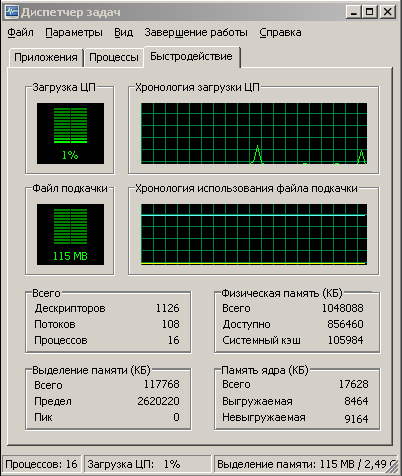
\includegraphics[width=.95\textwidth]{img/1}
  ReactOS
\end{minipage}%
\begin{minipage}{.5\textwidth}
  \centering
  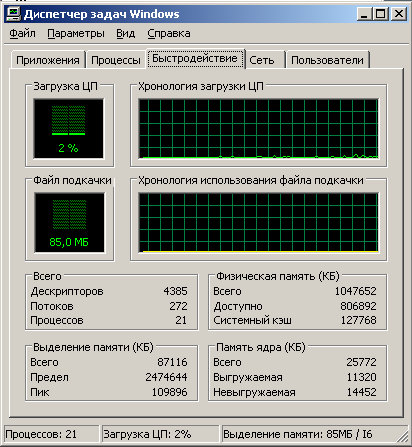
\includegraphics[width=.95\textwidth]{img/2}
  Windows 2003
\end{minipage}
\end{figure}
\end{frame}


\begin{frame}
\frametitle{История}
\vspace*{8em}
\begin{center}
\fullsizegraphic{img/history}
\end{center}
\end{frame}


\section{Архитектура}

\begin{frame}
\frametitle{Архитектура Windows NT}
\vspace*{1em}
\begin{center}
\fullsizegraphic{img/ntarch}
\end{center}
\end{frame}


\begin{frame}
\frametitle{Архитектура ReactOS}
\vspace*{1em}
\begin{center}
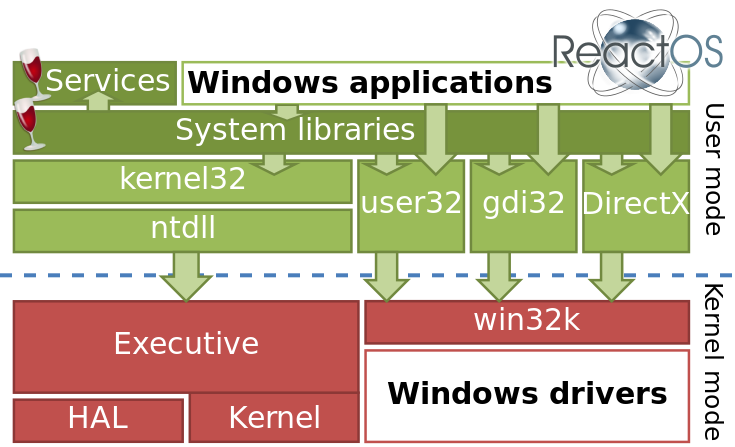
\includegraphics[width=\textwidth]{img/reactosarch}
\end{center}
\end{frame}


\begin{frame}
\frametitle{Wine и ReactOS}
ReactOS имеет много общего с Wine, благодаря своей открытости проекты поддерживают друг друга.
\textbf{Общие черты:}
\begin{itemize}
\item Установка приложений Windows;
\item Запуск приложений Windows.
\end{itemize}
\textbf{Отличия:}
\begin{itemize}
\item Работа на линуксе против работы на реальном железе;
\item Поддержка драйверов Windows.
\end{itemize}
\end{frame}


\begin{frame}
\frametitle{Kernel mode}

\textbf{HAL}(Hardware Abstraction Layer - Слой аппаратных абстракций) - позволяет запускать ОС на различных платах x86 без именений в ядре. Находится между аппаратным и програмными уровнями.

\textbf{win32k} - интерфейс для вывода информации(на монитор, принтер, другие устройства).

\textbf{Kernel}(NTOSKRNL) - микроядро, дизайн которого поддерживает различные архитектуры(x86-64, MIPS, Alpha...) реализует асинхронные вызовы процедур ядра (APC), вызовы отложенной процедуры (DPC), процессы, потоки, мьютексы, семафоры, блокировки...

Наиболее важные компоненты:
\begin{enumerate}
\item Планировщик;
\item Диспетчер;
\item Executive(исполнительная подсистема).
\end{enumerate}
\end{frame}

\begin{frame}
\frametitle{Планировщик}
Планировщик ядра NT - это планировщик на основе потоков, что означает, что он планирует потоки, а не процессы. 

Реализована вытесняющая многозадачность, при которой операционная система не ждет, когда поток сам захочет освободить процессор, а принудительно снимает его с выполнения после того, как тот израсходует отведенное ему время (квант), или если в очереди готовых появился поток с более высоким приоритетом.

Поддерживается 32 уровня приоритетов, разделенных на два класса - класс \textbf{реального времени} и \textbf{класс переменных приоритетов}. Потоки реального времени, приоритеты которых находятся в диапазоне от 16 до 31, являются более приоритетными процессами и используются для выполнения задач, критичных ко времени.
\end{frame}

\begin{frame}
\frametitle{Планировщик}
\vspace*{3em}
\begin{center}
\fullsizegraphic{img/schelder}
\end{center}
\end{frame}

\begin{frame}
\frametitle{Диспетчер}
Диспетчер - компонент ядра, который берёт на себя обработку объектов диспетчера, которые используются для синхронизации и оповещения. 
\begin{itemize}
\item \textbf{Событие} - Действие, начатое, как правило, вне рамок программы.
\item \textbf{Семафор} - Классический способ ограничения доступа к общим ресурсам.
\item \textbf{Поток} - Самая малая функциональная единица кода, выполняющегося на центральном процессоре.
\item \textbf{Таймер} - Счетчики, которые либо увеличиваются либо уменьшаются на определённой фиксированной частоте.
\item \textbf{Мьютекс} - Объект, позволяющий нескольким потокам получать синхронный доступ к ресурсам и избегать одновременного использования общих ресурсов.
\end{itemize}
\end{frame}

\begin{frame}
\frametitle{Executive(исполнительная подсистема)}
Executive(исполнительная подсистема) - подсистема, обеспечивающая драйверам высокоуровневый доступ к объектам диспетчера ядра, а также поддержку высокоуровневой функциональности процессов и потоков, такой, как маркеры (управляемые подсистемой защиты), объекты, дескрипторы, квоты, WIN32K, задания, порты (управляемые подсистемой вызова локальных процедур (LPC)) и т.д. 

Предоставляет несколько своих объектов, например быстрый мьютекс (fast mutex), обратные вызовы (callbacks), блокировки с заталкиванием указателя (pushlocks). 

Также, она предоставляет высокоуровневый доступ к некоторым структурам управления памятью и функциям, например, выделению пула.
\end{frame}

\begin{frame}
\frametitle{Сервисы Executive}
\textbf{Менеджер объектов(Object Manager)}
\begin{itemize}
\item Создает, удаляет и управляет объектами NT executive - абстрактными типами данных, используемых для представления ресурсов системы.
\end{itemize}
\textbf{Менеджер кэша}
\begin{itemize}
\item Реализация кэширования диска.
\end{itemize}
\textbf{Монитор безопасности}
\begin{itemize}
\item Устанавливает правила защиты на локальном компьютере. Охраняет ресурсы операционной системы, выполняет защиту и регистрацию исполняемых объектов.
\end{itemize}
\textbf{Менеджер процессов}
\begin{itemize}
\item Создает и завершает, приостанавливает и возобновляет процессы и нити, а также хранит о них информацию.
\end{itemize}
\end{frame}

\begin{frame}
\frametitle{Текущее положение}
\textbf{Хорошо}
\begin{itemize}
\item Планировщик, HAL, менеджер процессов и потоков.
\end{itemize}
\textbf{Еще требуется доработка}
\begin{itemize}
\item I/O подсистема, менджер конфигураций, менеджер безопасности.
\end{itemize}
\textbf{Плохо}
\begin{itemize}
\item Менеджер памяти, менеджер кэшей, библиотека поддержки файловой системы. Все три компонента так и небыли корректно реализованы с самого начала проекта.
\end{itemize}
\textbf{Не существует}
\begin{itemize}
\item Менеджер питания.
\end{itemize}
\end{frame}







\begin{frame}
\frametitle{Планы на ближайшее будущее}
\begin{itemize}
\item Совместимость с драйверами для NT 6.x (Vista/7/8/10)
\item Завершение поддержки печати
\item Безотказная работа ПО
\item Поддержка DirectX
\item Завершение реализации Wi-Fi
\item Исправление графических ошибок
\item Разметка дисковых разделов с использованием NTFS, exFAT,
\item Работа с SSD, RAID и составными томами напрямую.
\end{itemize}
\textbf{В далеком будущем}: выход из альфа версии, поддержка прочих архитектур.
\end{frame}

\begin{frame}
\frametitle{Интересные факты}
\begin{itemize}
\item Антивирусы активно использовали дыры(недокументированные API) в windows в следствии чего в reactOs для корректной работы их нужно специально эмулировать.
\item Когда в reactOs происходят сбои, их анализируют с помощью \textbf{WinDBG}, которая спрашивает хотите ли вы отправить данные в Microsoft, чтобы их проанализировали.
\item Пользователи по сути являются тестировщиками.
\item Данный проект позволяет заявить о себе.
\item Один из разработчиков \textbf{ReactOs} читал лекции \textbf{Windows} программистам о том как работает \textbf{Windows}.
\item Выдающиеся программисты ушли работать в \textbf{Microsoft} и другие крупные компании.
\item Также имеется "синий экран смерти".
\end{itemize}
\end{frame}


\begin{frame}[fragile]
\frametitle{Итоги}
\textbf{ReactOS} это:
\begin{itemize}
\item не Windows, это 100\% свободная и открытая реимплементация Windows;
\item не Linux, драйвера и программы работают нативно;
\item не Wine, от Wine используется лишь небольшая часть;
\item уникальный проект, которому требуется еще много работы.
\end{itemize}
\end{frame}	


\begin{frame}[fragile]
\frametitle{Курсовая работа}
\textbf{Идеи для работы:}
\begin{itemize}
\item Дополнить ReactOS(в ветку на гитхабе) новой функциональностью(много рисков).
\begin{itemize}
\item Высокая сложность, по большей части остался kernel mode.
\item Время на принятие дополнений в основную ветку.
\item Код ревью.
\item Риск, что кто-то другой это реализует.
\end{itemize}
\item Изменить поведение системы в той или иной мере.
\item В Jira проекта имеется список багов для исправлений. Взять один из багов, проанализировать причину его возникновения и попытаться исправить.
\end{itemize}
\end{frame}	

\begin{frame}
\frametitle{Список источников}
\begin{enumerate}
\item ReactOS Tech talk in Google Montreal by Alex Ionescu in 2013. - URL: https://www.youtube.com/watch?v=HNPoCz1IBoQ
\item Maraia, Vincent. (2005). The Build Master: Microsoft's Software Configuration Management Best Practices. 
\item ReactOS Kernel. URL: https://www.reactos.org/wiki/Kernel
\item ReactOS Ntoskrnl. URL: https://reactos.org/wiki/Ntoskrnl.exe
\item Build Environment. URL: https://winehq.org.ru/Build\_Environment
\item ReactOS GitHub. URL: https://github.com/reactos/reactos
\item ReactOS ports. URL: https://www.reactos.org/wiki/ReactOS\_ports
\item Концепции Windows NT. URL: http://citforum.ru/operating\_systems/sos/glava\_39.shtml
\item Концепции Windows NT. URL: http://rgata.ru/sites/mpoevs/uploads/cit-forum/operating\_systems/winntadm/winntadm\_01.html
\end{enumerate}
\end{frame}
	

	
\end{document}
